% https://tex.stackexchange.com/a/364080
\documentclass{beamer}

\usepackage{tikz}
\usetikzlibrary{arrows}
\usetikzlibrary{positioning}
\usetikzlibrary{matrix}


\begin{document}

\begin{frame}[fragile]
\begin{center}
    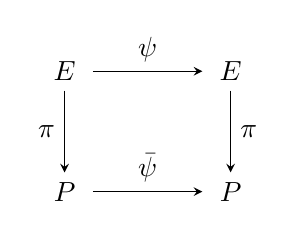
\begin{tikzpicture}
      \matrix (m) [matrix of math nodes,row sep=3em,column sep=4em,minimum width=2em]
      {
         E & E \\
         P & P \\};
      \path[-stealth]
        (m-1-1) edge node [left] {$\pi$} (m-2-1)
                edge node [above] {$\psi$} (m-1-2)
        (m-2-1.east|-m-2-2) edge node [below] {}
                node [above] {$\bar{\psi}$} (m-2-2)
        (m-1-2) edge node [right] {$\pi$} (m-2-2);
    \end{tikzpicture}  
\end{center}
\end{frame}

\end{document}
